\documentclass[12pt]{article}
\usepackage{amsmath}
\usepackage{graphicx}
\usepackage{float}
\usepackage{listings}
\usepackage{xcolor}
\usepackage{hyperref}

\begin{document}
%el documento consiste en una introduccion a el robot gekko, como interactuar con el y como programarlo
\title{Simulación}
\author{Team Mustabot 2022}
\date{\today}
%ahora introducimos los componentes del robot
\maketitle

\section*{Python}
\subsection{Condiciones}
en arduino(c++), para crear condiciones escribimos:
\begin{lstlisting}[language=C++]
    if(condicion){
        //codigo
    }
    else{
        //codigo
    }
\end{lstlisting}
en python, para crear condiciones escribimos:
\begin{lstlisting}[language=Python]
    if condicion:
        #codigo
    else:
        #codigo
\end{lstlisting}
En Python es sumamente importante la identación, esto pasa a ser nuestros nuevos corchetes {}. Además, ¡¡¡no necesitamos usar ; ni definir los tipos de variables!!!
para hacer un while en python:
\begin{lstlisting}[language=Python]
    while condicion:
        #codigo
\end{lstlisting}
para hacer un for en python:
\begin{lstlisting}[language=Python]
    for i in range(10):
        #codigo
\end{lstlisting}
\subsection{Funciones}
en arduino(c++), para crear funciones escribimos:
\begin{lstlisting}[language=C++]
    void nombre_funcion(int 1, int 2){
        //codigo
    }
\end{lstlisting}
en python, para crear funciones escribimos:
\begin{lstlisting}[language=Python]
    def nombre_funcion(parametro1, parametro2):
        #codigo
\end{lstlisting}

\subsection{Funciones predefinidas}
Ustedes trabajaran sobre un conjunto de funciones creadas para facilitar su aprendizaje y uso, de todas formas, ustedes pueden modificarlas
si quieren agregar una funcionalidad extra.
Siempre tendran la posibilidad de revisar todo el código y recordar como usar las funciones.
Aca hay en ejemplo de como estructurar el código del controlador del robot:
\begin{lstlisting}[language=Python]
    #importamos todos los ficheros
    def setup():
        #usamos variables globales
        global robot
        global leftMotor
        #redefinimos variables globales
        leftMotor = MOTOR(robot, "left motor")
    def loop():
        #usamos variables globales
        global leftMotor
        #usamos las funciones
        leftMotor.setVelocity(10)
\end{lstlisting}

A Continuación se muestra un ejemplo de el entorno de la simulación en el cual estarán trabajando
%\begin{figure}[H]
%    \centering
%    \includegraphics[width=0.9\textwidth=0.8]{simulacion_images/simulacion_robot.png}
%    \caption{Simulación}
%    \label{fig:simulacion}
%\end{figure}
\begin{figure}[H]
    \centering
    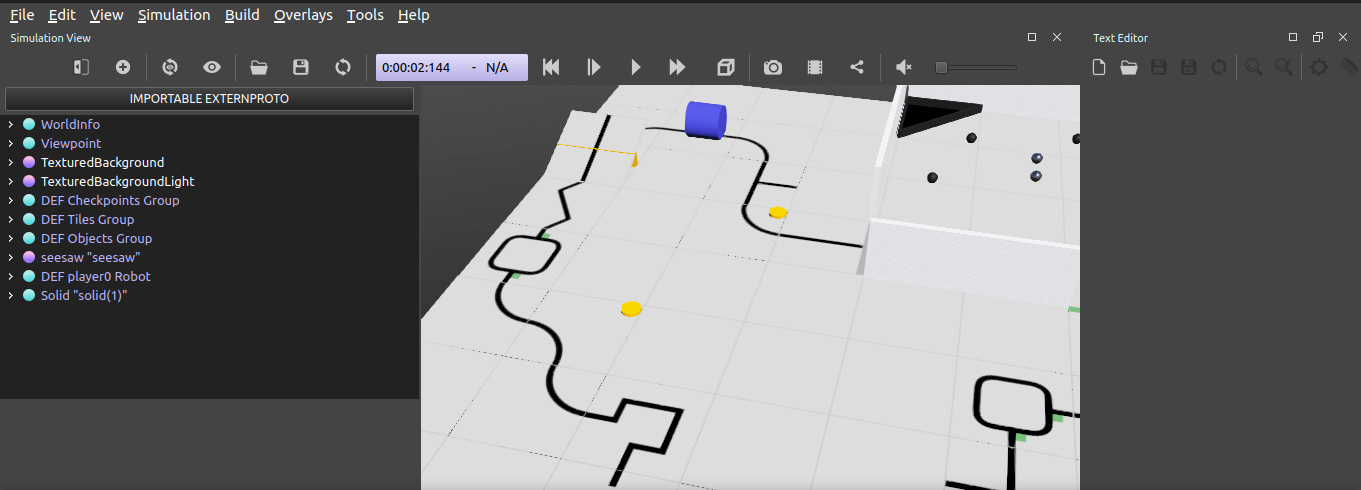
\includegraphics[width=0.9\textwidth=0.8]{simulacion_imagenes/simulacion_pista.png}
    \caption{Simulación}
    \label{fig:simulacion2}
\end{figure}

\section{Desafío}
El equipo tiene la misión de realizar un seguidor de lineas usando un PID, para esto, deberán realizar un código usando las funciones de movimiento y lectura de sensores que hemos visto durante esta clase.


Tutorial: como usar webots?
Documentacion: \href{https://cyberbotics.com/doc/guide/tutorial-1-your-first-simulation-in-webots?tab-language=python}{link a documentacion oficial}
Video: \href{https://www.youtube.com/watch?v=luyg3plGujg&list=PLbEU0vp_OQkUwANRMUOM00SXybYQ4TXNF}{link a video de apoyo}
%Documentacion: https://cyberbotics.com/doc/guide/tutorial-1-your-first-simulation-in-webots?tab-language=python
%adjuntamos un link
%Video: https://www.youtube.com/watch?v=luyg3plGujg&list=PLbEU0vp_OQkUwANRMUOM00SXybYQ4TXNF
%Tutorial: como usar gekko lib?
\end{document}